%\documentclass[notes]{beamer}       % print frame + notes
%documentclass[notes=only]{beamer}   % only notes
\documentclass{beamer}              % only frames

\usetheme{Copenhagen}
\usecolortheme{beaver}

\setbeamertemplate{navigation symbols}{}

\setbeamertemplate{frametitle}[default][center]

\usepackage{biblatex}
\bibliography{main}

\usepackage{hyperref}
\usepackage{minted}
\usepackage{amsmath}
\usepackage{multicol}
\usepackage{bibentry}

\usepackage{graphicx}
\usepackage{tikz}

\usetikzlibrary{calc, patterns}

\title{Equilibria Behaviour of Rational Agents}
\author{Vince Knight}
\date{}


\begin{document}

\frame{
    \titlepage
}

\section{knightva@cardiff.ac.uk}

\begin{frame}
    \frametitle{Auction}
        \begin{alertblock}{Dollar Auction}
            \centering
                Top two bids pay.
        \end{alertblock}
\end{frame}

\note{
    Invite audience to bid on a 5 bound note. Bids are by 10 pence.

    Explain that the winner of the auction WILL get the 5 pound note.

    Top two bids play.

    Once two individuals have started bidding they are caught in a cycle.

    1. Bids 4.80
    2. Bids 4.90

    1 will lose 4.80 if they do not bid. They will lose/win 0 if they bid 5.00.

    This leads to:

    1. Bids 5.00
    2. Bids 4.90

    Now 2 will lose 4.90 if they do not bid. 2 will lose .10 if they bid 5.00.
}

\begin{frame}
    \centering

    
\includegraphics[height=4cm]{static/CUident_CMYK.png}

\end{frame}

\section{Normal Form Games}

\begin{frame}

    \begin{definition}
        A $N$ player normal form game consists of:

        \begin{itemize}
            \item A finite set of $N$ players.
            \item Action set for the players: $\{\mathcal{A}_1, \mathcal{A}_2, \dots \mathcal{A}_N\}$
            \item Payoff functions for the players: $u_i : \mathcal{A}_1 \times \mathcal{A}_2 \dots \times \mathcal{A}_N \to \mathbb{R}$
        \end{itemize}
    \end{definition}
\end{frame}

\begin{frame}
    \begin{example}
        Two friends must decide what movie to watch at the cinema. Alice would like
        to watch a sport movie and Bob would like to watch a comedy. Importantly,
        they would both rather spend their evening together than apart.
    \end{example}
\end{frame}

\note{
    \begin{itemize}
        \item The finite set of \(N=2\) players are the two neighbouring
            countries.
        \item The action sets are \(\mathcal{A}_1=\mathcal{A}_2=\{\text{Sport}, \text{Comedy}\}\)
        \item For two player games a common representation of the payoff
            functions is:
            \[
                   A = \begin{pmatrix}
                   3 & 1\\
                   0 & 2
                   \end{pmatrix}
                   \qquad
                   B = \begin{pmatrix}
                   2 & 1\\
                   0 & 3
                   \end{pmatrix}
               \]
    \end{itemize}
}

\section{Strategies}

\begin{frame}
    \begin{definition}
        A strategy for a player with action set $\mathcal{A}$ is a probability
        distribution over elements of $\mathcal{A}$.
    
        Typically a strategy is denoted by $\sigma \in [0, 1]^{|\mathcal{A}|}_{\mathbb{R}}$ so that:
    
        $$\sum_{i=1}^{\mathcal{A}}\sigma_i = 1$$
    \end{definition}
\end{frame}

\note{
    As an example we have:

    \[\sigma_r=(1/7, 6/7)\qquad \sigma_c=(1, 0)\]

    This corresponds to Alice choosing sports \(\frac{1}{7}\) of the
    time and Bob unilaterally choosing to sports.
}

\begin{frame}
    \begin{definition}
        For a given strategy \(\sigma\), the support of \(\sigma\):
        \(\mathcal{S}(\sigma)\) is the set of actions \(i\in\mathcal{A}\) for
        which \(\sigma_i > 0\).
    \end{definition}
\end{frame}

\note{
    For our example we have:
    \[
        \mathcal{S}(\sigma_r=(1/7, 6/7))=\{\text{Sports}, \text{Comedy}\}
            \qquad
        \mathcal{S}(\sigma_c)=\{\text{Sports}\}
    \]
}


\begin{frame}
    \begin{definition}
    Average payoff:
        \begin{itemize}
            \item \(u_{r}(\sigma_r, \sigma_c) = \sigma_r A \sigma_c^T\)
            \item \(u_{c}(\sigma_r, \sigma_c)  = \sigma_r B \sigma_c^T\)
        \end{itemize}
    \end{definition}
\end{frame}

\note{
    For our example we have:
        \[
            \begin{aligned}
                u_{r}((1/7, 6/7), (1, 0))&=(1/7,6/7)\begin{pmatrix}3 &1\\
                                                               0&  2\\
                                                \end{pmatrix}\begin{pmatrix}1\\0\end{pmatrix}\\
                                         &=(1/7,6/7)\begin{pmatrix}3\\
                                                               0\\
                                                \end{pmatrix}\\
                                         &=\frac{3}{7} + \frac{0}{7}=\frac{3}{7}
            \end{aligned}
        \]
        and

        \[
            \begin{aligned}
                u_{r}((1/7, 6/7), (1, 0))&=(1/7,6/7)\begin{pmatrix}2&1\\
                                                               0 &  3\\
                                                \end{pmatrix}\begin{pmatrix}1\\0\end{pmatrix}\\
                                         &=(1/7,6/7)\begin{pmatrix}2\\
                                                               0\\
                                                \end{pmatrix}\\
                                         &=\frac{2}{7} + \frac{0}{7}=\frac{2}{7}
            \end{aligned}
        \]

    We see that Alice's utility is higher.
    This makes sense as Bob is choosing to no matter what: go see their
    favourite move.
}

\section{Best Responses}


\begin{frame}
    \begin{definition}
        In a two player game \((A,B)\in{\mathbb{R}^{m\times n}}^2\) a strategy
        \(\sigma_r^*\)  of the row player is a best response to a column players'
        strategy \(\sigma_c\) if and only if:

        \[\sigma_r^*=\text{argmax}_{\sigma_r\in \mathcal{S}_1}\sigma_rA\sigma_c^T\]
    \end{definition}
\end{frame}

\note{
    Let us compute the best response \(\sigma_r^*\) as a function of
                \(\sigma_c=(y, 1 - y)\).

    We have \(A\sigma_c =
                \begin{pmatrix}3y+1-y\\2(1-y)\end{pmatrix}=\begin{pmatrix}2y+1\\2-2y)\end{pmatrix}\)

    \begin{center}
        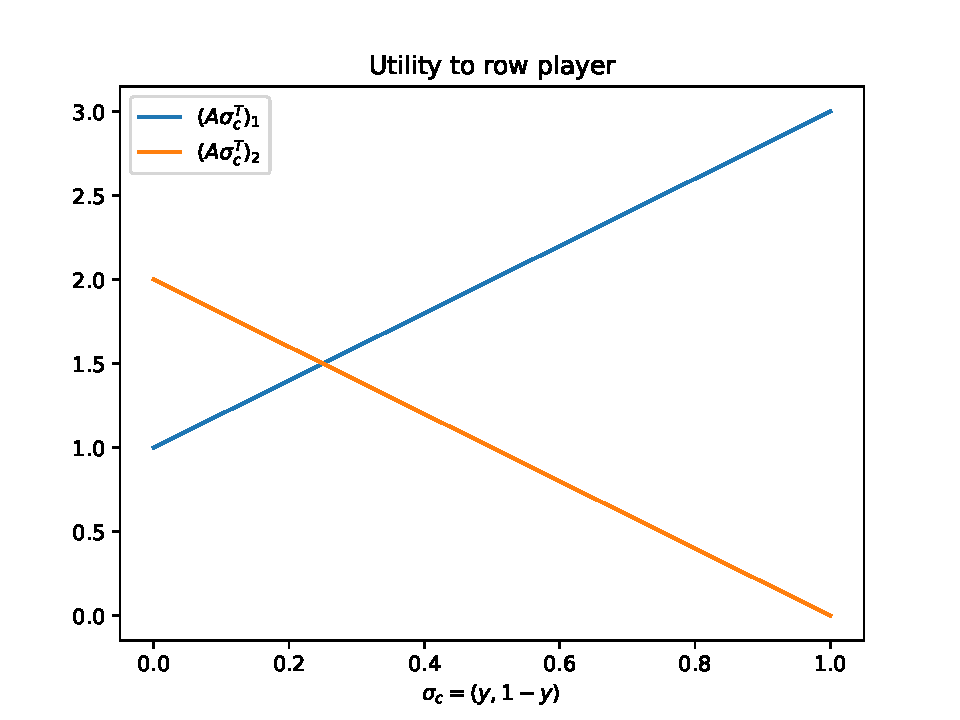
\includegraphics[width=3cm]{./static/best_response_plot_for_coordination_game/main.pdf}
    \end{center}


    This gives:
                \[
   \sigma_r ^* = \begin{cases}
                    (1, 0),& \text{ if } y < 1/4\\
                    (0, 1),& \text{ if } y > 1/4\\
                    \text{indifferent},& \text{ if } y=1/4
                 \end{cases}
                 \qquad
                 \text{similarly }
   \sigma_c ^* = \begin{cases}
                    (1, 0),& \text{ if } x > 3/4\\
                    (0, 1),& \text{ if } x < 1/4\\
                    \text{indifferent},& \text{ if } x=3/4
                 \end{cases}
             \]
}

\frame{
    \begin{theorem}
        In a two player game \((A,B)\in{\mathbb{R}^{m\times n}}^2\) a strategy
        \(\sigma_r^*\)  of the row player is a best response to a column players'
        strategy \(\sigma_c\) if and only if:

        \[
   {\sigma_{r^*}}_i > 0 \Rightarrow (A\sigma_c^T)_i = \text{max}_{k \in \mathcal{A}_2}(A\sigma_c ^ T)_k \text{ for all }i \in \mathcal{A}_1
\]
    \end{theorem}
}

\note{

    \tiny{
        \((A\sigma_c^T)_i\) is the utility of the row player when they play their
        \(i^{\text{th}}\) action. Thus:


        \[
            \sigma_rA\sigma_c^T=\sum_{i=1}^{m}{\sigma_r}_i(A\sigma_c^T)_i
        \]

        Let \(u=\max_{k}(A\sigma_c^T)_k\) giving:

        \begin{align}
            \sigma_rA\sigma_c^T&=\sum_{i=1}^{m}{\sigma_r}_i(u - u + (A\sigma_c^T)_i)\\
            &=\sum_{i=1}^{m}{\sigma_r}_iu - \sum_{i=1}^{m}{\sigma_r}_i(u - (A\sigma_c^T)_i)\\
            &=u - \sum_{i=1}^{m}{\sigma_r}_i(u - (A\sigma_c^T)_i)
        \end{align}

        We know that \(u - (A\sigma_c^T)_i\geq 0\), thus the largest
        \(\sigma_rA\sigma_c^T\) can be is \(u\) which occurs if and only if
        \({\sigma_r}_i > 0 \Rightarrow (A\sigma_c^T)_i = u\) as required.

    }
}

\frame{

    \centering
    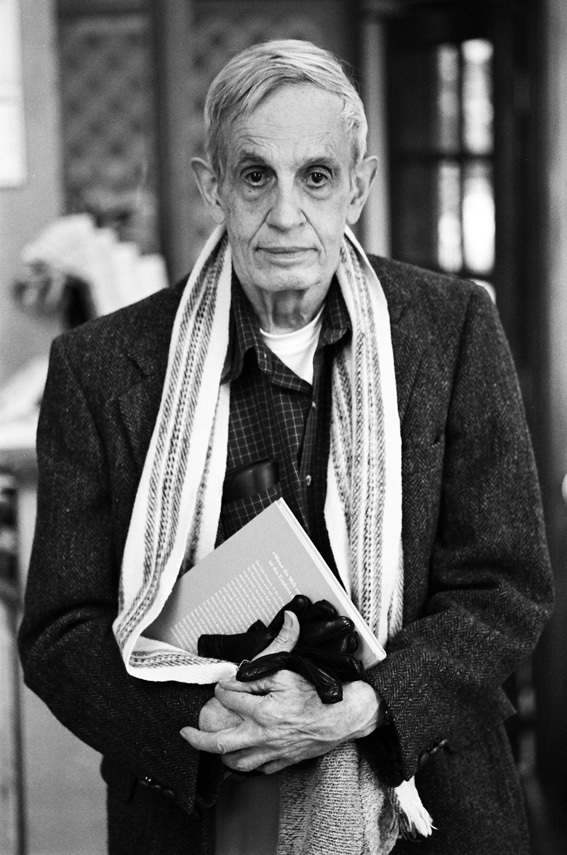
\includegraphics[height=.6\textheight]{./static/john-nash.jpg}

    \textbf{John Nash}\footfullcite{Nash1950} (1928 - 2015)


    \tiny{By Peter Badge / Typos1 - submission by way of Jimmy Wales, CC BY-SA
    3.0, \url{https://commons.wikimedia.org/w/index.php?curid=6977799}}

}

\note{
    In his 25 page PhD thesis John Nash proved the following theorem.

    \begin{theorem}
        All Normal Form games have a set of strategies that are best responses
        to each other.\footfullcite{Nash1950}
    \end{theorem}


    The proof is incredibly elegant. He shows, using Kakutani fixed point
    theorem from the field of topology that a fixed point exists for a function
    that corresponds to the equilibrium condition.

    \fullcite{kakutani1941generalization}
}


\section{Lemke Howson Algorithm}

\frame{
    \begin{definition}
        For a two player game $(A, B)\in{\mathbb{R}^{m\times n}_{>0}}^2$ the
        row/column player best response polytope $\mathcal{P}$/$\mathcal{Q}$ is
        defined by:

        \[
            \mathcal{P} = \left\{x\in\mathbb{R}^{m}\;|\;x\geq 0; xB\leq 1\right\}
        \]

        \[
            \mathcal{Q} = \left\{y\in\mathbb{R}^{n}\;|\; Ay\leq 1; y\geq 0 \right\}
        \]
    \end{definition}
}

\note{
    These best response polytopes is the bounded set of vectors that correspond
    to a scaled game where the best response of the row/column player is scaled
    to a value of 1.
}

\begin{frame}
        \centering
        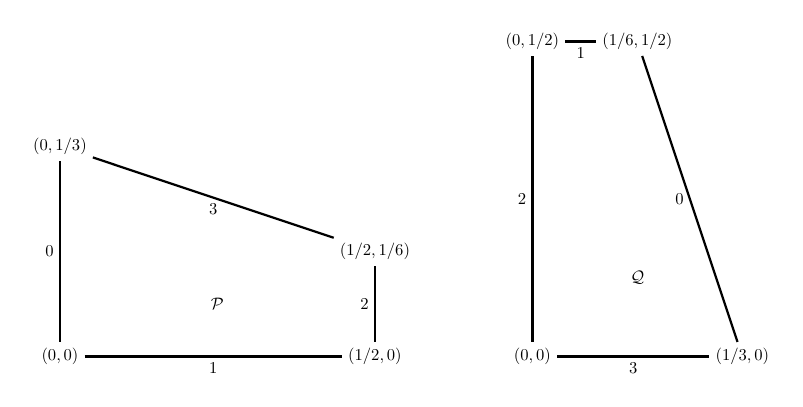
\begin{tikzpicture}[thick,scale=8, every node/.style={scale=0.6}]
            \node (a) at (0,0)  {\((0, 0)\)};
            \node (b) at (1/2, 0) {\((1/2, 0)\)};
            \node (c) at (0, 1/3) {\((0, 1/3)\)};
            \node (d) at (1/2, 1/6) {\((1/2, 1/6)\)};

            \draw (a) -- (b)  node[below, midway] {1};
            \draw (b) -- (d)  node[below, left, midway] {2};
            \draw (c) -- (d)  node[below, midway] {3};
            \draw (a) -- (c)  node[left, midway] {0};

            \node () at (1/4, 1/12) {\(\mathcal{P}\)};

            \node (a) at (3 / 4, 0)  {\((0, 0)\)};
            \node (b) at (13 / 12, 0) {\((1/3, 0)\)};
            \node (c) at (3 / 4, 1/2) {\((0, 1/2)\)};
            \node (d) at (11 / 12, 1/2) {\((1/6, 1/2)\)};

            \draw (a) -- (b)  node[below, midway] {3};
            \draw (b) -- (d)  node[below, left, midway] {0};
            \draw (c) -- (d)  node[below, midway] {1};
            \draw (a) -- (c)  node[left, midway] {2};

            \node () at (11 / 12, 1/8) {\(\mathcal{Q}\)};
        \end{tikzpicture}
\end{frame}

\note{
Here are the polytopes for our game.

We label the polytopes according to the ordered defining half spaces. Because of
the face that the ordering of \(\mathcal{P}\) and \(\mathcal{Q}\) we have a
correspondence between the vertices of the polytope. 

In \(\mathcal{P}\) the label $0$ corresponds to the first action of the row
player's actions not being played. However, in \(\mathcal{Q}\) the label \(0\)
corresponds to the first action of the row player being a best response.

}

\begin{frame}
        \centering
        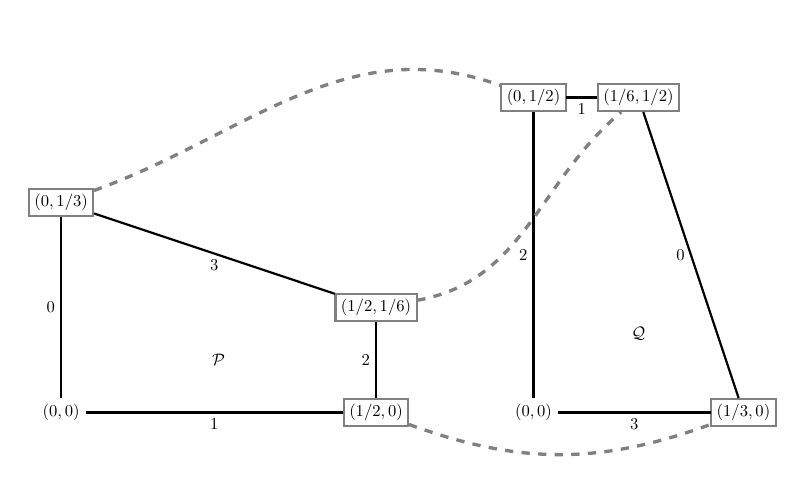
\begin{tikzpicture}[thick,scale=8, every node/.style={scale=0.6}]
            \node (p_a) at (0,0)  {\((0, 0)\)};
            \node (p_b) at (1/2, 0)  [draw=gray] {\((1/2, 0)\)};
            \node (p_c) at (0, 1/3)  [draw=gray] {\((0, 1/3)\)};
            \node (p_d) at (1/2, 1/6)  [draw=gray] {\((1/2, 1/6)\)};

            \draw (p_a) -- (p_b)  node[below, midway] {1};
            \draw (p_b) -- (p_d)  node[below, left, midway] {2};
            \draw (p_c) -- (p_d)  node[below, midway] {3};
            \draw (p_a) -- (p_c)  node[left, midway] {0};

            \node () at (1/4, 1/12) {\(\mathcal{P}\)};

            \node (q_a) at (3 / 4, 0)  {\((0, 0)\)};
            \node (q_b) at (13 / 12, 0) [draw=gray] {\((1/3, 0)\)};
            \node (q_c) at (3 / 4, 1/2) [draw=gray]  {\((0, 1/2)\)};
            \node (q_d) at (11 / 12, 1/2)  [draw=gray] {\((1/6, 1/2)\)};

            \draw (q_a) -- (q_b)  node[below, midway] {3};
            \draw (q_b) -- (q_d)  node[below, left, midway] {0};
            \draw (q_c) -- (q_d)  node[below, midway] {1};
            \draw (q_a) -- (q_c)  node[left, midway] {2};

            \node () at (11 / 12, 1/8) {\(\mathcal{Q}\)};

            \draw [very thick, color=gray, style=dashed] (p_b) [out=-20,in=200] to (q_b);
            \draw [very thick, color=gray, style=dashed] (p_c) [out=20,in=160] to (q_c);
            \draw [very thick, color=gray, style=dashed] (p_d) [out=10,in=220] to (q_d);
        \end{tikzpicture}
\end{frame}

\note{
    Once we have obtained the polytopes and labelled the vertices we can
    identify pairs of vertices (one in each polytope) that are \textbf{fully
    labeled}. A fully labeled vertex pair corresponds to pairs of strategies
    where either an action is not played or it is a best response to the
    strategies played by the other player.

    In this case we have a game with three pairs of fully labelled vertices.
    Which we can convert to strategies (ie probability vectors):

    \begin{itemize}
        \item \(\{(0, 1/3), (0, 1/2)\} \to \{(0, 1), (0, 1)\}\)
        \item \(\{(1/2, 0), (1/3, 0)\} \to \{(1, 0), (1, 0)\}\)
        \item \(\{(1/2, 1/6), (1/6, 1/2)\} \to \{(3/4, 1/4), (1/4, 3/4)\}\)
    \end{itemize}
}


\frame{
    \begin{block}{}
    Lemke-Howson Algorithm \footfullcite{Lemke1964}
    \end{block}
}

\note{
    The Lemke Howson Algorithm presents an approach to systematically search
    vertices in pairs.

    It allows us to unlock a technique called Integer Pivoting to efficiently
    find equilibria. Note however that it cannot guarantee to find all games.
}

\frame{
    \begin{block}{}
    A game theoretic model of the behavioural gaming that takes place at the EMS - ED interface\footfullcite{panayides2023}
    \end{block}
    \centering
    
\includegraphics[width=.6\textwidth]{./static/ems-ed.jpg}
}

\note{
There are a number of examples of applications of Nash equilibria.

In this paper, we modelled the interface of emergency units and emergency
vehicles. Ambulances are often blocked with patients because hospitals do not
want to start a timer of taking them in the door. This blocks ambulances.

There are limitations to Nash equilibria: does the equilibria actually arise?
This will be the topic of my next seminar.
}

\frame{
    \begin{center}
        \huge
        \url{nashpy.readthedocs.io}

        \url{knightva@cardiff.ac.uk}
    \end{center}
}

\end{document}

